\documentclass{beamer}
\usepackage[export]{adjustbox}
\usepackage{graphicx}
\definecolor{mygreen}{rgb}{.125,.5,.25}
\usecolortheme[named=mygreen]{structure}


\usetheme{Warsaw}


\title{Komunikator Internetowy "Chatter"}
\author{Przemysław Jaroszkiewicz}
\institute{Akademia Górniczo-Hutnicza im.Stanisława Staszica}
\date{}

\begin{document}

\begin{frame}
 \titlepage
\end{frame}

\begin{frame}{Temat Prezentacji}
 \begin{enumerate}
  \item Socket'y i komunikacja Client-Server
  \item Komunikacja grupowa
  \item MySQL Server
  \item MySQL Database
 \end{enumerate}
\end{frame}



\begin{frame}{Socket Client-Server}
 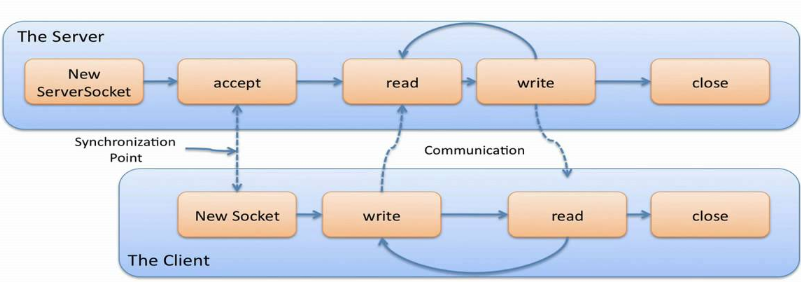
\includegraphics[scale=0.5]{socket_overview}
\end{frame}



\begin{frame}{Server Side}
Stworzenie serwera:
 \begin{figure}[h]
  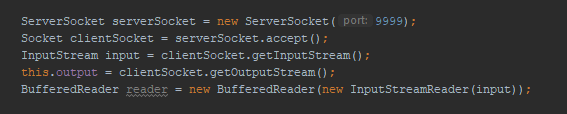
\includegraphics[scale=0.5]{server_code}

 \end{figure}
Wypisanie połaczenia w konsoli:
 \begin{figure}
  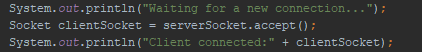
\includegraphics[width=.6\textwidth,left]{server_write}
 \end{figure}

 \begin{figure}
  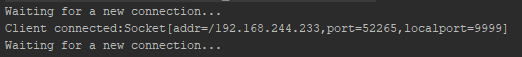
\includegraphics[width=.6\textwidth,left]{server_console}
 \end{figure}
\end{frame}




\begin{frame}{Przyjmowanie wielu połaczeń}
\begin{figure}
 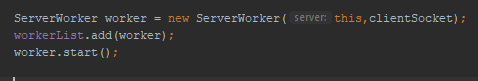
\includegraphics[scale=0.8]{serverWorker}
\end{figure}
\begin{figure}
 \centering
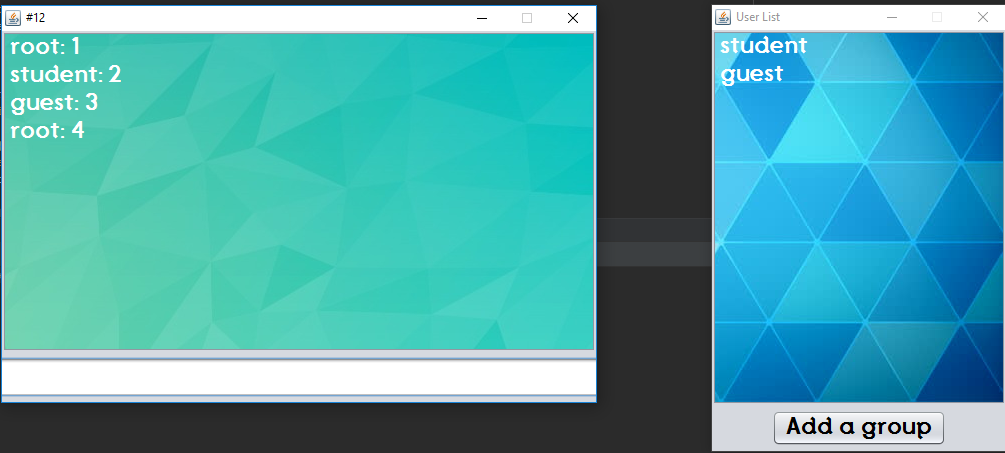
\includegraphics[scale=0.4]{grp}
\end{figure}
\end{frame}






\begin{frame}{Komendy}
 Tokeny i rozpoznawanie komend przez serwer
\begin{figure}
 \centering
  \begin{minipage}[b]{0.5\textwidth}
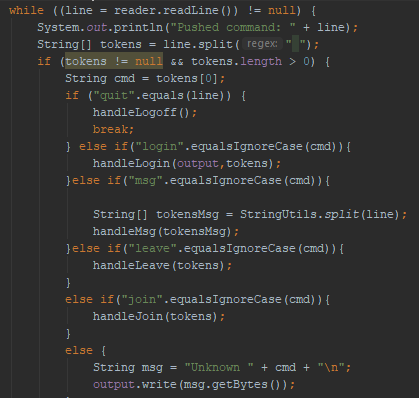
\includegraphics[width=\textwidth,left]{server_command}
\end{minipage}
  \hfill
  \begin{minipage}[b]{0.5\textwidth}
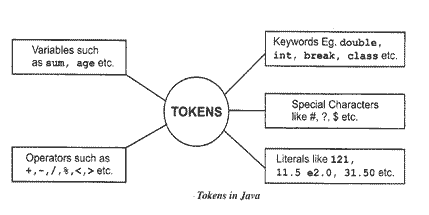
\includegraphics[width=\textwidth,right]{tokens}
 \end{minipage}
\end{figure}
\end{frame}


\begin{frame}{Telnet}
\begin{figure}
 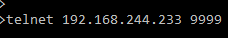
\includegraphics[scale=1]{telnet}
\end{figure}
\begin{figure}
 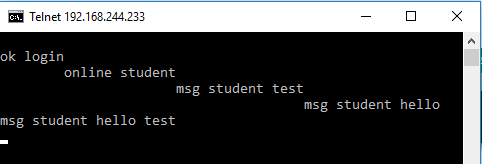
\includegraphics[scale=0.5]{msg_telnet}
\end{figure}
\begin{figure}

 \centering
  \begin{minipage}[b]{0.4\textwidth}
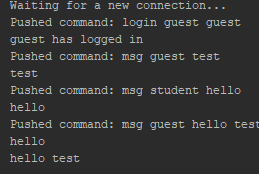
\includegraphics[width=\textwidth,left]{msg_console}
\end{minipage}
  \hfill
  \begin{minipage}[b]{0.4\textwidth}
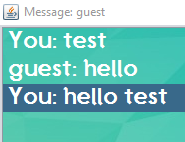
\includegraphics[width=\textwidth,right]{msg_app}
 \end{minipage}
\end{figure}
\end{frame}



\begin{frame}{Aplikacja - Client side}
\begin{figure}
 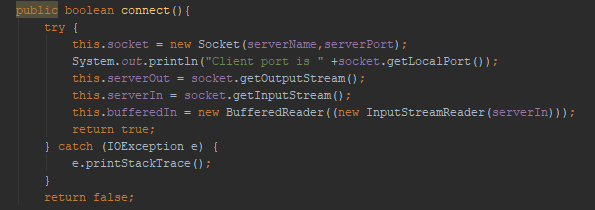
\includegraphics[scale=0.5]{client_socket}
\end{figure}
\begin{figure}

 \centering
  \begin{minipage}[b]{0.48\textwidth}
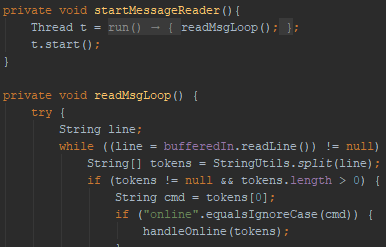
\includegraphics[width=\textwidth,left]{client_read}
\end{minipage}
  \hfill
  \begin{minipage}[b]{0.48\textwidth}
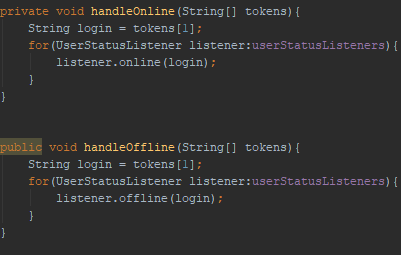
\includegraphics[width=\textwidth,right]{client_handle}
 \end{minipage}
\end{figure}
\end{frame}



\begin{frame}{Aplikacja - Listeners}

\begin{figure}
\centering
  \begin{minipage}[b]{0.3\textwidth}
\raisebox{+0.5\height}{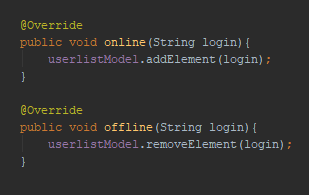
\includegraphics[width=\textwidth,left]{listener_online}}
\end{minipage}
  \hfill
  \begin{minipage}[b]{0.65\textwidth}
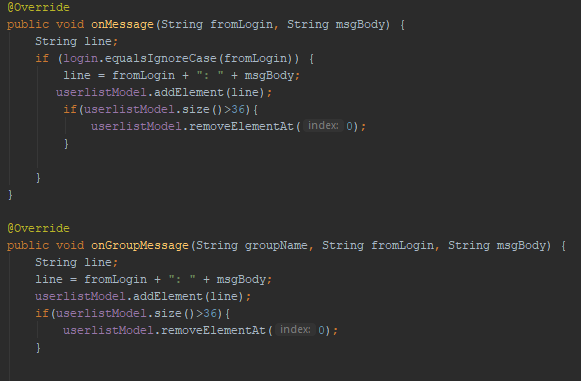
\includegraphics[width=\textwidth,right]{listener_msg}
 \end{minipage}
\end{figure}
\end{frame}


\begin{frame}{Aplikacja}
\begin{figure}
\centering
  \begin{minipage}[b]{0.7\textwidth}
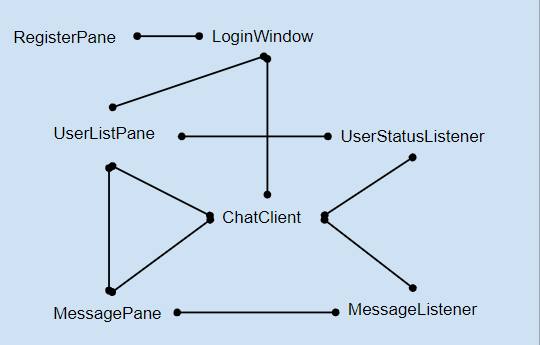
\includegraphics[width=\textwidth,left]{app1}
Client
\end{minipage}
  \begin{minipage}[b]{0.28\textwidth}
\raisebox{+0.04\height}{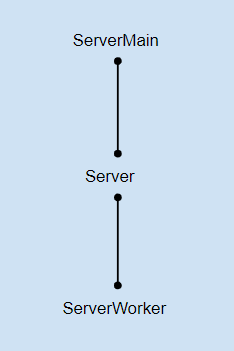
\includegraphics[width=\textwidth,right]{app2}}
Server
 \end{minipage}
\end{figure}
\end{frame}

\begin{frame}{MySQL Database}
 
\includegraphics[scale=0.5]{mysql}
\end{frame}



\begin{frame}{MySQL Server}
\begin{figure}
 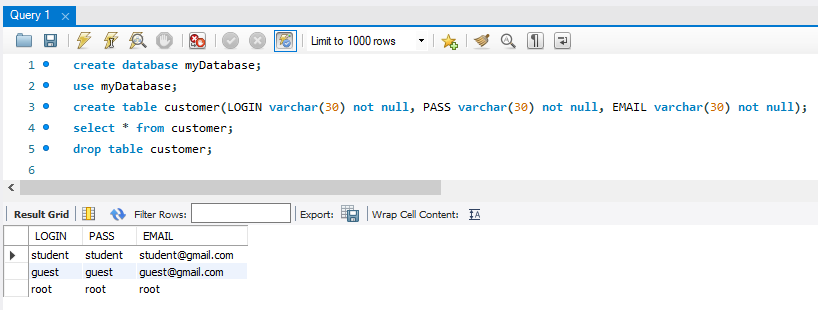
\includegraphics[scale=0.5]{mysql_server}
\end{figure}
\end{frame}



\begin{frame}{MySQL Client}
\begin{figure}
 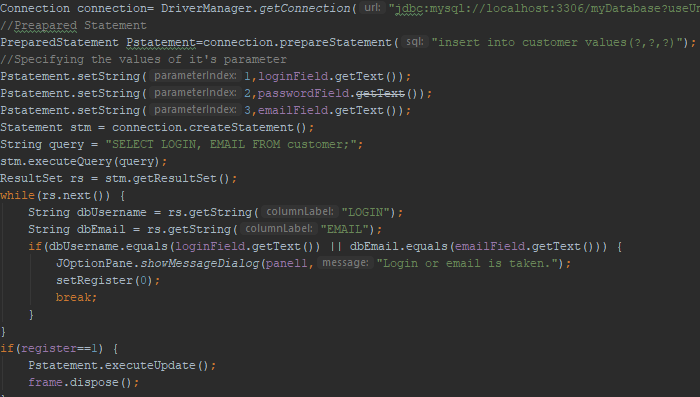
\includegraphics[scale=0.5]{mysql_connection}
\end{figure}
\end{frame}










\end{document}